\documentclass[a4paper]{article}

\usepackage[T1]{fontenc}
\usepackage[utf8]{inputenc}
\usepackage[brazilian]{babel}
%\usepackage{concrete}
\usepackage{lmodern}
\usepackage{amsmath,amssymb,amsfonts,amscd}
\usepackage{mathtools}
\usepackage{xcolor}
\usepackage{enumerate}
\usepackage{verbatim}
\usepackage{emerald}
\usepackage{fancybox}
\usepackage{booktabs}
\usepackage{fancyhdr}
	\pagestyle{fancy}
		\lhead{Guia do Usuário}
		\chead{}
		\rhead{\rightmark}
\usepackage{tikz}
\usepackage{esint}
\usepackage{esvect}
\usepackage{multicol}
\usepackage[most,listings]{tcolorbox}
\usepackage{hyperref}
	\hypersetup{colorlinks=true,linkcolor=blue,urlcolor=blue,}
\usepackage{comment}
\usepackage{graphicx}
\usepackage[labelfont=bf,font=small]{caption}
\usepackage{setspace}
%%%%%%%%%%%%%%%%%%%%%%%%%%%%%%%%%%%%%%%%%%%%%%%%%%%%%%%%%%%%%%%%%%%%%%%%%%%%%%%%%%%%%
\DeclareMathOperator{\sen}{sen}
\DeclareMathOperator{\tg}{tg}
\DeclareMathOperator{\cossec}{cossec}
\DeclareMathOperator{\cotg}{cotg}
\DeclareMathOperator{\arcsen}{arcsen}
\DeclareMathOperator{\arctg}{arctg}
\DeclareMathOperator{\arcsec}{arcsec}
\DeclareMathOperator{\Ln}{Ln}
\DeclareMathOperator{\Arg}{Arg}
\DeclareMathOperator{\cis}{cis}
%%%%%%%%%%%%%%%%%%%%%%%%%%%%%%%%%%%%%%%%%%%%%%%%%%%%%%%%%%%%%%%%%%%%%%%%%%%%%%%%%%%%%

%==================================================================================================================
% Simbolos e Atalhos Úteis
%==================================================================================================================
\newcommand{\vf}{(\quad)}
\newcommand{\vazio}{\varnothing}%--------------------> Símbolo do Vazio
\newcommand{\dd}{\,\mathrm{d}}%----------------------> texto romano para o ``d'' das derivadas 
\newcommand{\intc}{\varointctrclockwise}%------------> Integral para curva fechada do sentido anti-horário
\newcommand{\Resp}[1]{\hfill {\footnotesize\textbf{Resp.}:\;\,#1}}%--> Coloca ``Resposta'' no final de cada item.
\newcommand{\versor}[1]{\cdot\vec{\textbf{#1}}}%------------------------------> vetor em negrito
\newcommand{\alterdce}[5]{\begin{enumerate}%-------------------------------------> Alternativas em duas colunas
	\begin{minipage}{0.45\linewidth}
			\item #1
			\item #2
			\item #3
	\end{minipage}
	\hfill
	\begin{minipage}{0.45\linewidth}
			\item #4
			\item #5
	\end{minipage}
\end{enumerate}
}
\newcommand{\altercols}[6]{%----------------> alternativas em colunas (quantas quiser): nº de colounas + 5 itens.
\begin{multicols}{#1}\begin{enumerate}\item{#2} \item{#3} \item{#4} \item{#5} \item{#6}\end{enumerate}\end{multicols}}
%==================================================================================================================

\newenvironment{Atividade}[1]{%
\noindent
\newcounter{quest}
	\begin{list}{\ovalbox{\textbf{Questão \arabic{quest}.}}}{\usecounter{quest}
	\setlength{\labelwidth}{-2mm} \setlength{\parsep}{0mm}
	\setlength{\topsep}{0mm} \setlength{\leftmargin}{0mm}}
	\renewcommand{\labelenumi}{(\alph{enumi})}
	\newcommand{\questao}{\item}
	\onehalfspacing
	#1
	}{\end{list}}
	
\newenvironment{itens}{%
\begin{enumerate}
}{\end{enumerate}}
%---------------------------------------------------------------------------------

\newtcolorbox{codbox}[1]{%
box align=top,
colback=white,
colframe=gray!90,
breakable,
fonttitle=\bfseries,
title= #1
}

\begin{comment}
\begin{tcblisting}{colback=red!5!white,colframe=red!75!black}
This is a \LaTeX\ example:
\begin{equation}
\sum\limits_{i=1}^n i = \frac{n(n+1)}{2}.
\end{equation}
\end{tcblisting}


\begin{tcblisting}{colback=red!5!white,colframe=red!75!black,listing side text,
  title=Side by side,fonttitle=\bfseries}
This is a \LaTeX\ example:
\begin{equation}
\sum\limits_{i=1}^n i = \frac{n(n+1)}{2}.
\end{equation}
\end{tcblisting}
\end{comment}
%---------------------------------------------------------------------------------
	
\title{\textbf{Guia do Usuário}\\ \Large\{\texttt{\textcolor{red}{\textbf{ativmatUFRB.cls}}}\}}
\author{Ícaro Vidal Freire\thanks{Professor Assistente I da Área de Matemática do Centro de Formação de Professores (CFP) da Universidade Federal do Recôncavo da Bahia (UFRB).\newline \emph{e-mail}: \href{mailto:icarofreire@ufrb.edu.br}{icarofreire@ufrb.edu.br}}}
\date{\normalsize{\texttt{Versão~1.6}}\\ \small{\texttt{20/03/2020}}}

\begin{document}
\maketitle
\begin{abstract}
Este é um pequeno guia para utilização da classe, \texttt{ativmatUFRB.cls}, para \textcolor{red}{\textbf{ativ}}idades do curso de licenciatura em \textcolor{red}{\textbf{mat}}emática da \textcolor{red}{\textbf{UFRB}}.
\end{abstract}

\tableofcontents
%

\section{Antes de começar\ldots}
	\subsection{Versão}
	A primeira versão da classe \texttt{ativmatUFRB.cls}, a saber, \texttt{v~1.6}, foi concluída em 20/03/2020. A ideia é fazer a versão convergir ao número de ouro. Toda estruturação é derivada da classe padrão do \LaTeX\ denominada \texttt{article.cls}. Apenas foi acrescentado um cabeçalho estilizado com o logotipo da UFRB e informações sobre o título da lista, professor, disciplina, curso, semestre e número da lista; bem como comandos internos que julgamos úteis na construção de uma lista com questões de matemática ou física.
	\subsection{Projeto de Extensão \LaTeX\ CFP}
	A motivação para desenvolver esta classe vem do \emph{Projeto de Extensão}, cadastrado no Centro de Formação de Professores, intitulado: \emph{\LaTeX\ para o Professor de Matemática}. Tal projeto é ofertado (parcialmente) em forma de curso que versa sobre a confecção de materiais didáticos impressos (e também visuais – como apresentações) com alta qualidade tipográfica usando o programa \LaTeX, bem como no desenvolvimento de classes extra-oficiais (lista de atividade, avaliações, trabalho de conclusão de curso, etc.) para o curso de Licenciatura ou Bacharelado em Matemática da UFRB.
	
\section{Como instalar?}
Na pasta intitulada \emph{Classe para Atividade UFRB} estão:
\begin{description}
\item[Modelo.tex] Modelo de Lista de Atividade que explora os comandos internos da classe. Nesse arquivo também há comentários (marcados com \%) para auxilio dos usuários.
\item[ativmatUFRB.cls] A classe em si, ou seja, o conjunto de modificações que implementam as necessidades básicas de uma lista de atividade com cabeçalho estilizado para a \textsc{ufrb}. 
\item[Pasta ``Figuras''] Uma pasta que contém o logotipo\footnote{há também outras figuras que foram usadas como exemplo na lista. Estas podem ser descartadas depois.} da \textsc{ufrb} utilizado no cabeçalho (que não deve ser deletado). Caso sua lista de atividade contenha figuras, estas devem ser colocadas exclusivamente nesta pasta.
\end{description}

É aconselhável não modificar o arquivo \texttt{ativmatUFRB.cls}. Por isso, é importante armazená-lo em local apropriado. Salvar cada atividade em uma pasta é fundamental para a organização pessoal. Por exemplo, suponha que seja construída uma primeira lista de atividade de certa disciplina. Cria-se uma pasta intitulada ``Lista 01\_Tema da Lista''. Nessa pasta deve conter uma outra pasta, ``Figuras'', com o logotipo da UFRB e outras figuras usadas em questões da lista; e, pelo menos, o arquivo \texttt{Modelo.tex} (que pode ter outro nome, claro. Geralmente o mesmo da pasta principal ``\texttt{Lista 01\_Tema da Lista.tex}''). Feito isso, existem, de uma forma geral, dois modos para armazenar o arquivo \texttt{ativmatUFRB.cls}:

\subsection{Modo não aconselhável}
Um primeiro modo é deixar o arquivo \texttt{ativmatUFRB.cls} na mesma pasta onde se encontra o arquivo \texttt{Modelo.tex}, ou seja, na pasta ``Lista 01\_Tema da Lista''. Assim, toda vez que for preciso fazer uma outra lista, deve-se copiar o arquivo \texttt{ativmatUFRB.cls} novamente. Além disso, corre-se o risco de apagar esse arquivo mais facilmente.
\subsection{Modo aconselhável}
Uma forma mais conveniente é colocar o arquivo \texttt{.cls} em um local de acesso mais restrito (para evitar que se apague com facilidade) e que não seja preciso copiar todas as vezes que for necessária a criação de uma nova lista, ou seja, seria conveniente, ao compilar o arquivo \texttt{.tex}, que o MiK\TeX, automaticamente, encontrasse o arquivo \texttt{.cls}. Para tanto, deve-se criar uma pasta, por exemplo, ``ativmatUFRB-cls'', no disco local $C$. Especificamente, no seguinte caminho:

\begin{center}
\Ovalbox{\begin{minipage}{0.8\linewidth}
C: $\rightarrow$ Arquivos de Programas $\rightarrow$ MiKTeX 2.9 $\rightarrow$ tex $\rightarrow$ latex 
\end{minipage}
}
\end{center}

Depois disso é necessário atualizar o console do MiK\TeX\ da seguinte maneira:
\begin{enumerate}
	\item[(1)] Localize o \emph{MiK\TeX\ Console (Admin)}: ou digitando na barra de pesquisa de seu computador, ou pelo caminho:
	\begin{center}\ovalbox{\begin{minipage}{0.6\linewidth} C:\,$\rightarrow$\,MiKTeX 2.9\,$\rightarrow$\, miktex \,$\rightarrow$\, bin \,$\rightarrow$\, x64 \end{minipage}}\end{center}
	\item[(2)] Ao conceder as permissões para acessar o console, clique em 
	\begin{center}\ovalbox{\begin{minipage}{0.5\linewidth}\emph{Tasks} \,$\rightarrow$\, \emph{Refresh file name database}\end{minipage}}\end{center}
\end{enumerate}

\begin{figure}[!htbp]
\centering
\caption{Depois de criar uma pasta no diretório do MiK\TeX\, no \texttt{disco C}, é necessário uma atualização no banco de dados}
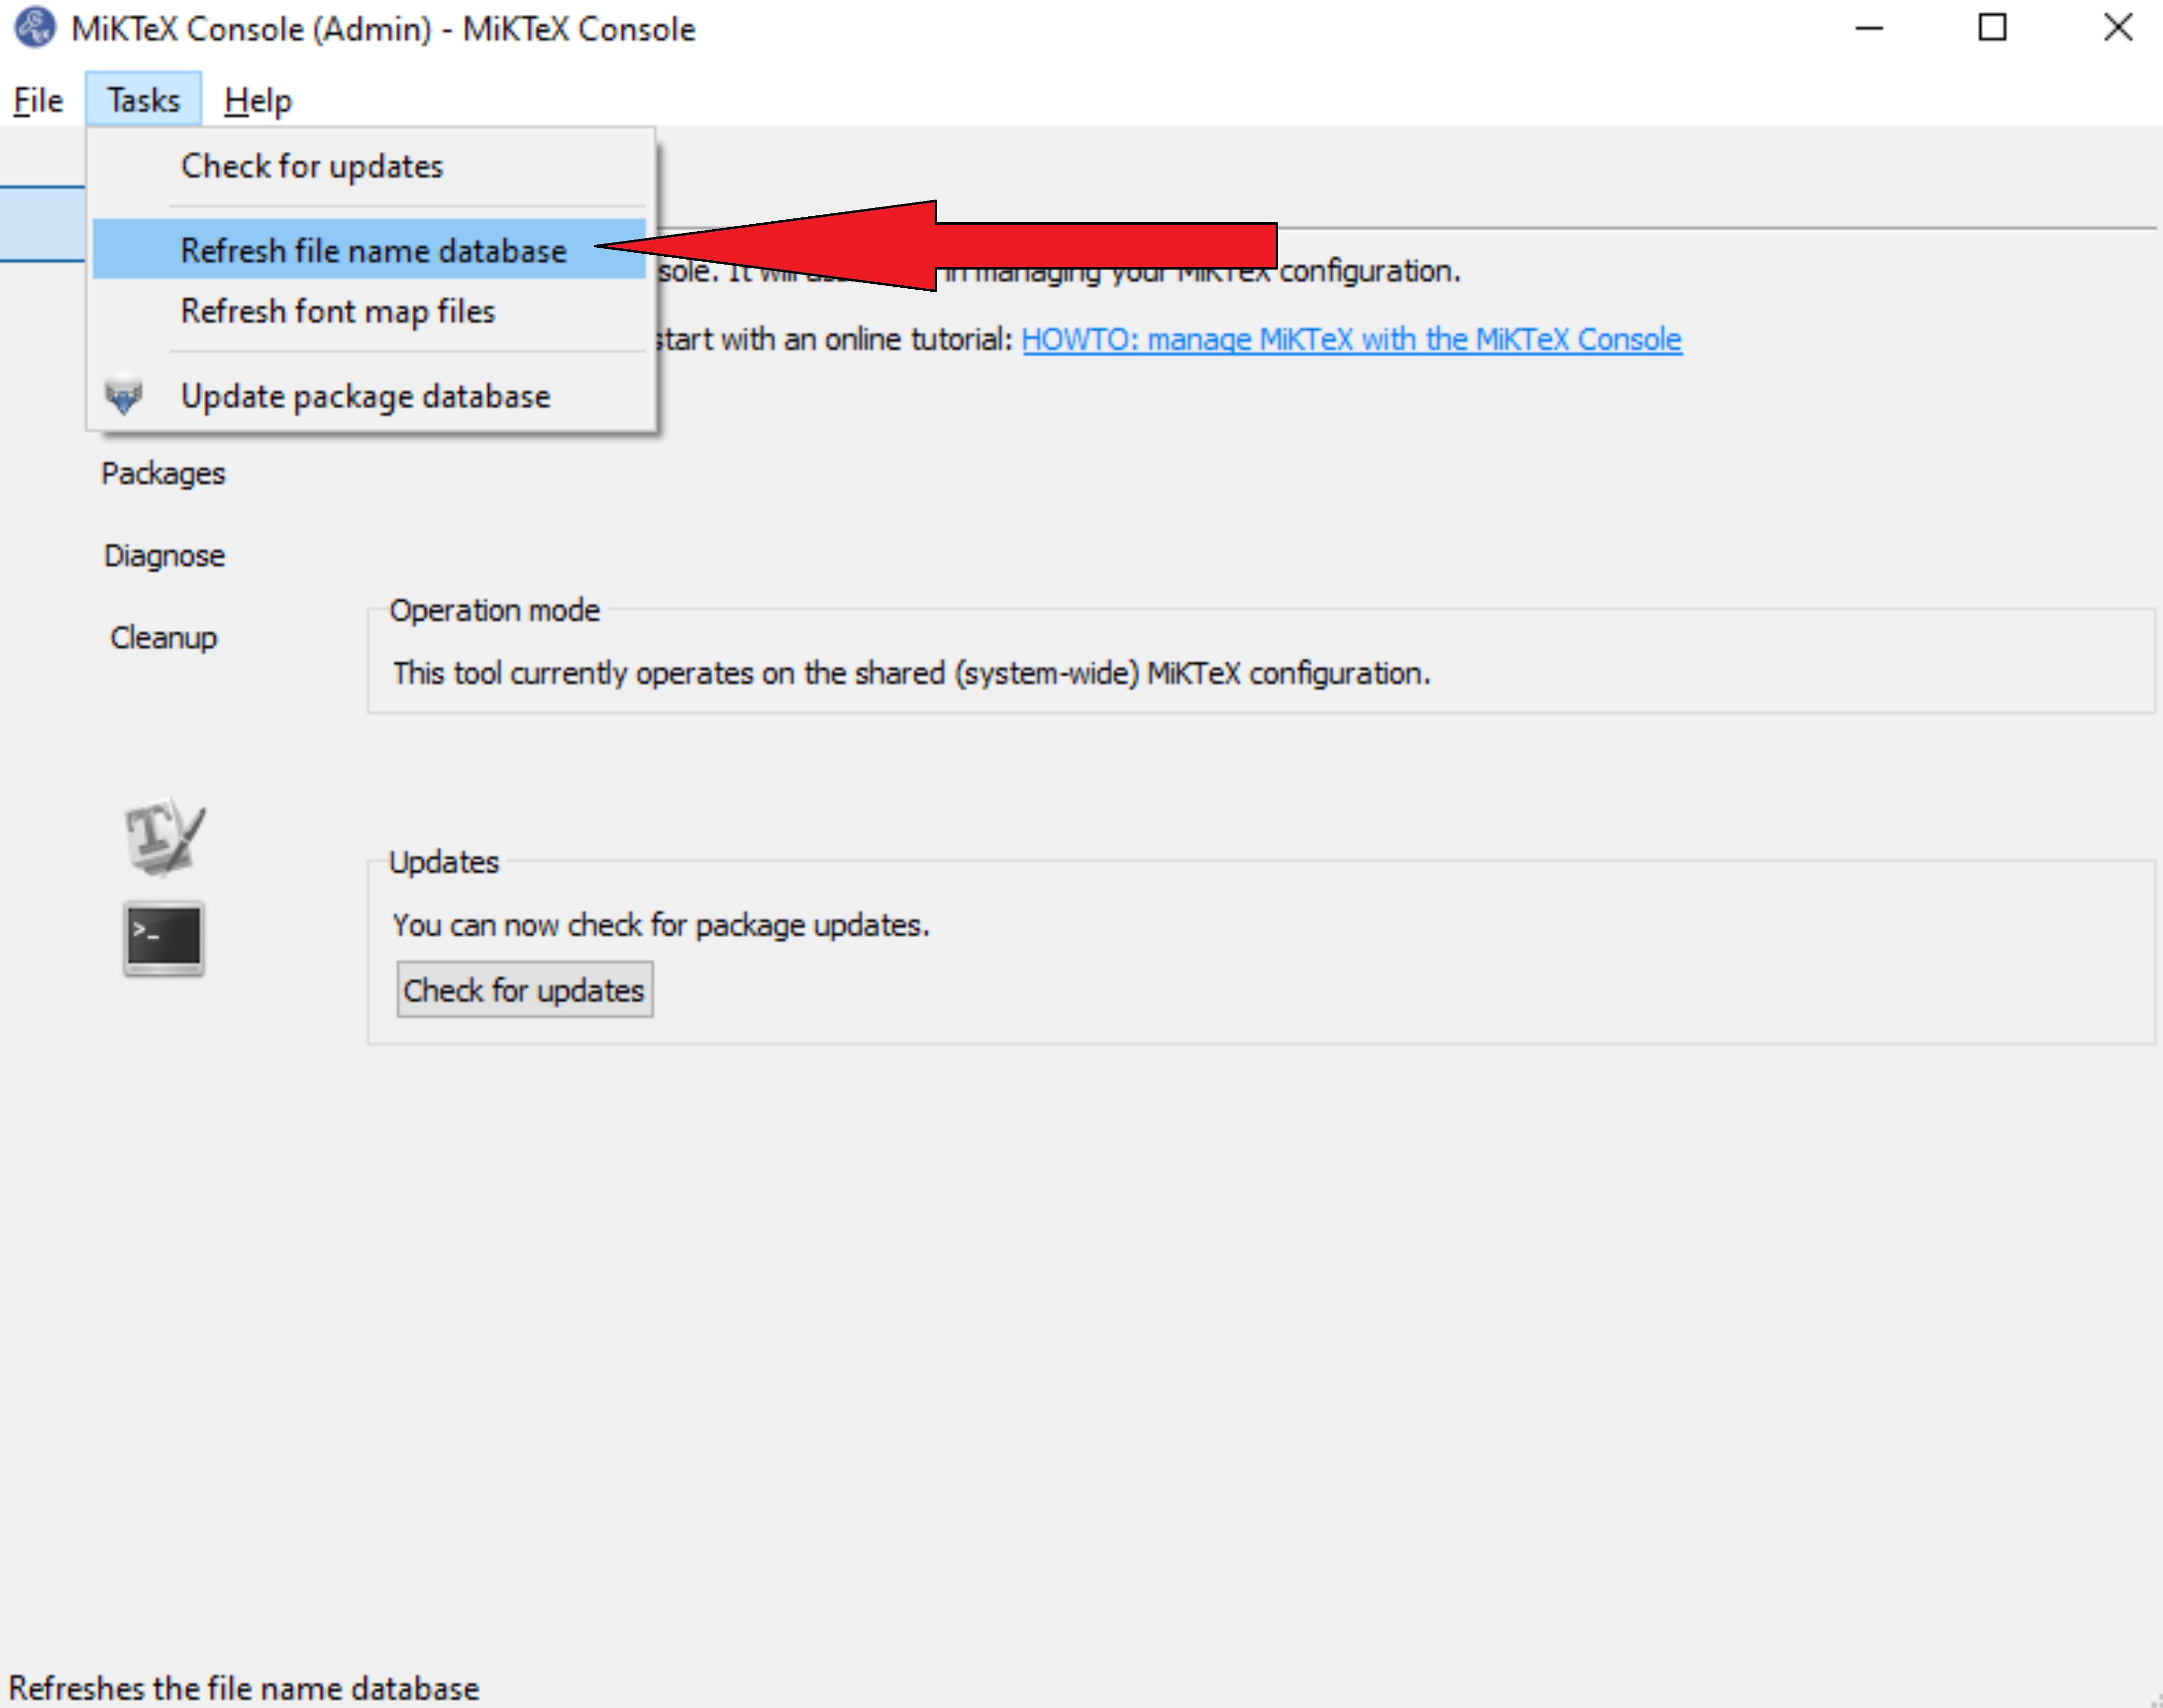
\includegraphics[width=0.9\textwidth]{MiKTeX}
\label{fig:MiKTeX}
\end{figure}

\section{Explicando a classe \texttt{ativmatUFRB.cls}}
Abaixo estão os comandos criados nessa classe para confecção das listas de atividade.

\subsection{\texttt{\textbackslash titulo}}
Esse comando deve ser colocado logo após o \verb|\begin{document}|. Ele gera um cabeçalho estilizado, com logotipo da UFRB; e, é composto de seis itens obrigatórios, a saber:
\begin{enumerate}[(i)]
	\item \verb|\TituloDaLista{}|. Escreva o título da sua lista de atividade;
	\item \verb|\Prof{}|. O nome do professor da disciplina;
	\item \verb|\Disciplina{}|. A disciplina referente à lista, por exemplo, \emph{Funções de uma Variável Complexa}, \emph{Cálculo I}, etc.
	\item \verb|\Curso{}|.  Curso onde está alocada a disciplina, por exemplo, \emph{Licenciatura em Matemática}, etc.
	\item \verb|\Semestre{}|. Semestre onde se encontra a disciplina, por exemplo, $2^{\circ}$~semestre. Nesse caso, coloque \textbf{apenas} o numeral associado. No caso do exemplo citado, deverá ser feito assim: \verb|\Semestre{2}|.
	\item \verb|\NumeroDaLista{}|. O número da lista deve ser colocado em \textbf{algarismos romanos}. Por exemplo, se for a primeira lista, deve ser escrito assim: \verb|\NumeroDaLista{I}|.
\end{enumerate}

Os seis itens citados acima devem ser colocados no preâmbulo do documento, ou seja, entre o \verb|\documentclass{ativmatUFRB}| e o \verb|\begin{document}|.

\begin{codbox}{Exemplo de preenchimento do comando \texttt{\textbackslash titulo}}
\begin{verbatim}
\documentclass{ativmatUFRB}
%=======================================
% Informações do Título da Lista
%=======================================
\TituloDaLista{Título da Lista}
\Prof{Ícaro Vidal Freire}
\Disciplina{Cálculo Vetorial e Integral}
\Curso{Licenciatura em Matemática}
\Semestre{2}
\NumeroDaLista{I}
%=======================================
\begin{document}
\titulo %------> Comando para o cabeçalho
...
\end{document}
\end{verbatim}
\end{codbox}

%
\subsection{Ambiente para Questões}
%
O ambiente \verb|\begin{Atividade} ...\end{Atividade}| enumera uma lista com o nome ``Questões'' estilizado: texto em negrito, dentro de uma caixa oval, sem ``indentação''. Usamos assim:

\begin{tcblisting}{colback=blue!5!white,colframe=blue!70!black,listing side text, title=Ambiente para ``Questões'',fonttitle=\bfseries}
\begin{Atividade}
\questao Primeira questão.
\questao Segunda questão.
\end{Atividade}
\end{tcblisting}

Note que para cada ``Questão estilizada'', usamos o comando \verb|\questao|. Na Subseção~\ref{comand} falaremos sobre comandos para escrever dois tipos de alternativas nesse ambiente, cada uma com 5~(cinco) itens. 

%
\subsection{Ambiente para alternativas gerais}
%
Os comandos \verb|\begin{itens}...\end{itens}| produz um ambiente propício para os ``itens'' (alternativas) dentro do ambiente \texttt{Atividade}. Para produzir cada item, usamos o comando \verb|\item|.

\begin{tcblisting}{colback=blue!5!white,colframe=blue!70!black,listing side text, title=Ambiente geral para alternativas,fonttitle=\bfseries}
\begin{Atividade}
\questao Início da questão.
\begin{itens}
\item Primeiro item.
\item Segundo item.
\end{itens}
\end{Atividade}
\end{tcblisting}

Você pode usar esse ambiente para produzir inúmeras listas, bastando para isso colocar, entre \textit{colchetes}, o primeiro elemento da lista desejada. A classe \texttt{ativmatUFRB.cls} fornece o comando \verb|\vf| para produzir um espaço em branco entre dois \textit{parenteses}, \vf, para ser usado, por exemplo, em questões que envolvam ``\textcolor{red}{v}erdadeiro'' ou ``\textcolor{red}{f}also''. 

\begin{tcblisting}{colback=blue!5!white,colframe=blue!70!black,listing side text,title=Lista em romano (minúscula),fonttitle=\bfseries}
\begin{Atividade}
\questao Início da questão.
\begin{itens}[(i)]%1º elem. da lista entre [] 
\item Primeiro item.
\item Segundo item.
\end{itens}
\end{Atividade}
\end{tcblisting}

\begin{tcblisting}{colback=blue!5!white,colframe=blue!70!black,listing side text,title=Lista em Romano (maiúscula),fonttitle=\bfseries}
\begin{Atividade}
\questao Início da questão.
\begin{itens}[(I)]
\item Primeiro item.
\item Segundo item.
\end{itens}
\end{Atividade}
\end{tcblisting}

\begin{tcblisting}{colback=blue!5!white,colframe=blue!70!black,listing side text,title=Lista para ``verdadeiro'' ou ``falso'',fonttitle=\bfseries}
\begin{Atividade}
\questao Início da questão.
\begin{itens}[\vf]
\item Primeiro item.
\item Segundo item.
\end{itens}
\end{Atividade}
\end{tcblisting}

%
\subsection{Operadores matemáticos}
%
Funções trigonométricas podem ser digitadas diretamente no idioma pt-BR. Algumas funções foram omitidas: ou por já serem contempladas no idioma inglês\footnote{na realidade estão disponíveis nos pacotes da $\AmS$ (\textit{American Mathematical Society}). Falaremos sobre ele na Seção~\ref{pacotes}, mas adiantamos que funções como $\arg,\, \ln,\, \cos,$ etc., já se encontram no pacote citado.} (como \verb|\cos{}|, por exemplo), ou por não serem tão recorrentes (por exemplo, \verb|\arccossec{}|). Neste último caso, se for necessário, escreva no preâmbulo do seu texto o operador diretamente (no exemplo, acima exposto, pode ser obtido por: \verb|\DeclareMathOperator{\arccossec}{arccossec}|). A Tabela~\ref{tab:op} exibe os Operadores matemáticos disponíveis na classe \texttt{ativmatUFRB.cls}:

\begin{table}[!htbp]
\centering
\caption{Tabela com os Operadores da classe \texttt{ativmatUFRB.cls}}
\label{tab:op}
\begin{tabular}{lcl}
\toprule
\textbf{Operador} && \textbf{Saída}\\
\midrule
\verb|\sen| && $\sen{}$\\
\verb|\tg| && $\tg$\\
\verb|\cossec| && $\cossec$\\
\verb|\cotg| && $\cotg$\\
\verb|\arcsen| && $\arcsen$\\
\verb|\arctg| && $\arctg$\\
\verb|\arcsec| && $\arcsec$\\
\verb|\Ln| && $\Ln$\\
\verb|\Arg| && $\Arg$\\
\verb|\cis| && $\cis$\\
\bottomrule
\end{tabular}
\end{table}

%
\subsection{\texttt{\textbackslash topico\{\}} \& Cia}
%
Caso queira acrescentar tópicos, subtópicos ou até mesmo ``subsubtópicos'' entre blocos de questões, basta usar os respectivos comandos:
\verb|\topico{}|, \verb|\subtopico{}| e \verb|\subsubtopico{}|. Apenas o comando \verb|\topico{}| produz uma faixa cinza que engloba o título da seção desejada. Os outros deixam as subseções e ``subsubseções'' em negrito com diminuição da fonte (como na classe \verb|article.cls|).


%
\subsection{Comandos úteis}\label{comand}
%
A classe \texttt{ativmatUFRB.cls} disponibiliza alguns comandos úteis para construção de listas de atividade para matemática.
Obviamente os comandos não são exaustivos, visto que cada professor possui suas particularidades nas disciplinas.

\subsubsection*{\textbackslash \texttt{vazio}}
O comando \verb|\vazio| produz o símbolo do conjunto vazio, $\varnothing$.
\subsubsection*{\textbackslash \texttt{dd}}
Digitando \verb|\dd| em um ambiente matemático produzirá $\dd$, ou seja, a letra ``d'' usada como símbolo da diferencial (com um pequeno espaço antes do mesmo). Por exemplo, numa integral em função da variável $x$, note a diferença sutil:
\begin{tcblisting}{colback=blue!5!white,colframe=blue!70!black,listing side text, title=$\dd$ vs $d$,fonttitle=\bfseries}
$\displaystyle \int f(x)\dd{x}$ 
\\
$\displaystyle \int f(x) dx$
\end{tcblisting}

\subsubsection*{\textbackslash \texttt{intc}}
O simbolo para a integral de linha de uma curva fechada orientada no sentido anti-horário, $\displaystyle \intc$,  é dado pelo pacote \texttt{esint} através do comando, não tão atrativo para a língua portuguesa, \verb|\varointctrclockwise|. Na presente classe, o mesmo símbolo pode ser obtido usando \verb|\intc| (lembre de ``\textcolor{red}{\textbf{int}}egral no sentido \textcolor{red}{\textbf{c}}ontrário ao relógio'').
\subsubsection*{\textbackslash \texttt{versor}}
Suponha que você queira escrever algum vetor unitário em negrito e com o sinal do produto escalar usual, então basta usar o comando \verb|\versor{}|. 

\begin{tcblisting}{colback=blue!5!white,colframe=blue!70!black, title=Vetores unitários em negrito com o sinal do ``produto'',fonttitle=\bfseries}
$\vv{F}(x,y,z)= L(x,y)\versor{i}+M(x,y)\versor{j}+N(x,y)\versor{k}$
\end{tcblisting}
\subsubsection*{\textbackslash \texttt{Resp}}
Geralmente os alunos gostam de saber a resposta final de alguma questão para comparar com a resposta encontrada por eles. Nesta classe, usamos o comando \verb|\Resp{}| para criar um ambiente com fonte menor, localizado sempre à direita, onde aparece o texto ``Resp.:'' em negrito. Veja um exemplo abaixo:

\begin{tcblisting}{colback=blue!5!white,colframe=blue!70!black, title=Resposta alinhada à direita,fonttitle=\bfseries}
Seja $\mathcal{D}$ a parte da coroa circular compreendida entre $x^2+y^2=1$ e $x^2+y^2=4$ no primeiro quadrante.
Calcule \[\iint\limits_{\mathcal{D}}(x^2+y^2)\,dx\,dy\] \Resp{$15\pi/8$}
\end{tcblisting}

\subsubsection*{\textbackslash \texttt{altercols}}
Para uma lista de alternativas, o ambiente padrão \texttt{itens} servirá adequadamente. Entretanto, frequentemente, deseja-se construir uma lista com cinco alternativas de resposta (onde uma está correta). Para isso, usamos o comando \verb|\altercols{}{}{}{}{}{}| dentro do ambiente \verb|\begin{Atividade}|. Perceba que esse comando possui 6~(seis) parâmetros: o primeiro é o número de colunas que pretende-se dividir as alternativas; e, os outros cinco parâmetros são as alternativas. Por isso o nome do comando ``\textcolor{red}{\textbf{alter}}nativas em \textcolor{red}{\textbf{col}}una\textcolor{red}{\textbf{s}}''. É obrigatório especificar os 6 (seis) parâmetros. Obviamente, o primeiro parâmetro (número de colunas) varia de 1 a 5.

\begin{tcblisting}{colback=blue!5!white,colframe=blue!70!black, title=Alternativas em 5 colunas,fonttitle=\bfseries}
\begin{Atividade}
\questao Uma questão qualquer.
\altercols{5}{0}{1}{2}{3}{4}
\end{Atividade}
\end{tcblisting}

\begin{tcblisting}{colback=blue!5!white,colframe=blue!70!black, listing side text, title=Alternativas em 2 colunas,fonttitle=\bfseries}
\begin{Atividade}
\questao Uma questão qualquer.
\altercols{2}{0}{1}{2}{3}{4}
\end{Atividade}
\end{tcblisting}


\subsubsection*{\textbackslash \texttt{alterdce}}
Observe que no exemplo anterior, especificamente naquele em que se desejou escrever as alternativas em 2~(duas) colunas, houve um espaço vertical não tão conveniente entre as alternativas (d) e (e). Para sanar esse problema, devemos usar o comando \verb|\alterdce{}{}{}{}{}|.
Note que só há 5~(cinco) parâmetros (todos dever ser preenchidos com as alternativas), pois não há variação no número de colunas (duas colunas fixas). Assim, caso você queira ``\textcolor{red}{\textbf{alter}}nativas em \textcolor{red}{\textbf{d}}uas \textcolor{red}{\textbf{c}}olunas \textcolor{red}{\textbf{e}}specíficas'', faça como no exemplo:

\begin{tcblisting}{colback=blue!5!white,colframe=blue!70!black, title=Alternativas em 2 colunas específicas,fonttitle=\bfseries}
\begin{Atividade}
\questao Uma questão qualquer.
\alterdce{0}{1}{2}{3}{4}
\end{Atividade}
\end{tcblisting}

%
\section{Lista de pacotes já instalados}\label{pacotes}
%
A classe \texttt{ativmatUFRB.cls} já contém alguns pacotes básicos para contrução de uma lista de atividade em matemática. Listamos todos os pacotes dessa classe abaixo. Caso você precise de algum outro pacote, deve inseri-lo no preâmbulo do arquivo \texttt{.tex}.

\subsection*{\texttt{\textbackslash usepackage[explicit]\{titlesec\}}}
Esse pacote fornece uma interface para modificar/vriar comandos para seleção de vários estilos de título. Veja a documentação para mais detalhes:\\ {\small\url{http://linorg.usp.br/CTAN/macros/latex/contrib/titlesec/titlesec.pdf}}
\subsection*{\texttt{\textbackslash usepackage[T1]\{fontenc\}}}
Pacote para codificação de saída de fonte. Com ele, ocorre corretamente a hifenação das diversas fontes possivelmente usadas no texto.\\
{\small\url{https://www.ctan.org/pkg/fontenc}}
\subsection*{\texttt{\textbackslash usepackage[utf8]\{inputenc\}}}
Pacote para codificação de entrada. Dentre outras coisas, permite a acentuação diretamente pelos caracteres do nosso teclado. \emph{É obrigatório que seu arquivo \texttt{.tex} esteja salvo em codificação \textsc{utf8}}.\\
{\small\url{http://linorg.usp.br/CTAN/macros/latex/base/inputenc.pdf}}
\subsection*{\texttt{\textbackslash usepackage[brazilian]\{babel\}}}
Este pacote gerencia regras tipográficas (e outras) culturalmente determinadas para uma ampla variedade de idiomas. Por exemplo, traduz elementos internos de diversas classes \textit{standart} do \LaTeX.\\
{\small\url{http://linorg.usp.br/CTAN/macros/latex/required/babel/base/babel.pdf}}
\subsection*{\texttt{\textbackslash usepackage\{geometry\}}}%[a4paper,top=1cm,bottom=1.5cm,outer=1.5cm,inner=1.5cm]
O pacote fornece uma interface de usuário fácil e flexível para personalizar o layout da página. No caso da nossa classe, usamos a saída para papel A4, com margem superior de 1cm e as outras com 1.5cm.\\
{\small\url{http://linorg.usp.br/CTAN/macros/latex/contrib/geometry/geometry.pdf}}
\subsection*{\texttt{\textbackslash usepackage\{lmodern\}}}
Uma família de fontes Latim Modern que produz o ``corpo de texto'' da classe \texttt{ativmatUFRB.cls}.\\
{\small\url{https://www.ctan.org/tex-archive/fonts/lm/}}
\subsection*{\texttt{\textbackslash usepackage\{emerald\}}}
\emph{Emerald} é um pacote que dá suporte a algumas fontes gratuitas ECF (\emph{Emerald City Fontwerks}) no \LaTeX. Ela foi usada para produzir, de forma estilizada, o nome {\ECFIntimacy Lista de Atividade \ldots} no cabeçalho.\\
{\small\url{http://linorg.usp.br/CTAN/fonts/emerald/doc/emerald.pdf}}
\subsection*{\texttt{\textbackslash usepackage\{lipsum\}}}
Este pacote oferece acesso fácil ao texto fictício do \emph{Lorem Ipsum}, separando-o em parágrafos. Serve para testes tipográficos com palavras que simulam uma escrita mais adequada do que repetições de palavras (como ``texto, texto, texto'').\\
{\small\url{http://linorg.usp.br/CTAN/macros/latex/contrib/lipsum/lipsum.pdf}}
\subsection*{\texttt{\textbackslash usepackage\{amsmath,amsthm,amsfonts,amssymb,amscd\}}}
Diversos pacotes da Sociedade Americana de Matemática (\emph{American Mathematical Society}). Os pacotes \AmS-\TeX\ são fundamentais para escrita matemática. Segue a documentação de cada um deles:
\begin{description}
	\item[amsmath] Para diversos comandos de escrita matemática.\\ {\small\url{http://linorg.usp.br/CTAN/macros/latex/required/amsmath/amsldoc.pdf}}
	\item[amsthm]  Para configurações de teoremas, corolários, etc.\\ {\small\url{http://linorg.usp.br/CTAN/macros/latex/required/amscls/doc/amsthdoc.pdf}}
	\item[amsfonts] Diversos símbolos e fontes\footnote{veja uma tabelas mais resumida: \url{http://milde.users.sourceforge.net/LUCR/Math/mathpackages/amsfonts-symbols.pdf}}. Por exemplo, produz a simbologia características de conjuntos numéricos ($\mathbb{N}$ é produzido com o comando \verb|$\mathbb{N}$|).\\ {\small\url{http://linorg.usp.br/CTAN/fonts/amsfonts/doc/amsfndoc.pdf}}
	\item[amssymb] Diversos símbolos matemáticos\footnote{veja esse \emph{link} para visualização mais rápida: \url{https://www.rpi.edu/dept/arc/training/latex/LaTeX_symbols.pdf}}.\\	{\small\url{http://texdoc.net/texmf-dist/doc/fonts/amsfonts/amssymb.pdf}}
	\item[amscd] Pacote para criar diagramas comutativos\footnote{veja também o pacote tikz: \url{http://ctan.math.washington.edu/tex-archive/graphics/pgf/contrib/tikz-cd/tikz-cd-doc.pdf}}\\		{\small\url{http://linorg.usp.br/CTAN/macros/latex/required/amsmath/amscd.pdf}}
\end{description}
\subsection*{\texttt{\textbackslash usepackage\{mathtools\}}}
O \emph{Mathtools} fornece muitas ferramentas úteis para a composição matemática. Ele é baseado no \texttt{amsmath} e corrige várias deficiências desde e do \LaTeX\ padrão. {\small\url{http://linorg.usp.br/CTAN/macros/latex/contrib/mathtools/mathtools.pdf}}
\subsection*{\texttt{\textbackslash usepackage\{systeme\}}}
Pacote para construir sistemas de equações.\\{\small\url{http://linorg.usp.br/CTAN/macros/generic/systeme/systeme_fr.pdf}}
\subsection*{\texttt{\textbackslash usepackage\{esint\}}}
Para produzir diversos tipos de integrais.\\ {\small\url{http://linorg.usp.br/CTAN/macros/latex/contrib/esint/esint-doc.pdf}}
\subsection*{\texttt{\textbackslash usepackage\{array\}}} %\setcounter{MaxMatrixCols}{20}
Pacote para construção e modificação de diversos parâmetros numa tabela. A classe \texttt{ativmatUFRB.cls} está programada para um limite de 20 colunas numa tabela,  \verb|\setcounter{MaxMatrixCols}{20}|.\\ {\small\url{http://linorg.usp.br/CTAN/macros/latex/required/tools/array.pdf}}
\subsection*{\texttt{\textbackslash usepackage\{esvect\}}}
Essencial para produzir vetores. \\ {\small\url{http://linorg.usp.br/CTAN/macros/latex/contrib/esvect/esvect.pdf}}
\subsection*{\texttt{\textbackslash usepackage\{graphicx\}}} %\graphicspath{{./Figuras/}}
Dentre outras funcionalidades, esse pacote é essencial para inserção de figuras e ambiente para estas num documento. A classe \texttt{ativmatUFRB.cls} foi coonfigurada para que as figuras sejam buscadas na pasta ``Figuras'' (usou-se o comando \verb|\graphicspath{{./Figuras/}}|). Portanto, \textbf{todas} as figuras da lista de atividade devem estar numa pasta intitulada ``Figuras''. \\{\small\url{http://linorg.usp.br/CTAN/macros/latex/required/graphics/grfguide.pdf}}
\subsection*{\texttt{\textbackslash usepackage[table]\{xcolor\}}}
Produz inúmeras cores\footnote{veja exemplos com \texttt{pstricks}: \url{http://linorg.usp.br/CTAN/macros/latex/contrib/xcolor/xcolor2.pdf}} estilizadas.\\ {\small\url{http://linorg.usp.br/CTAN/macros/latex/contrib/xcolor/xcolor.pdf}}
\subsection*{\texttt{\textbackslash usepackage\{enumerate\}}}
Implementa modificações em ambientes com listas enumeradas. \\ {\small\url{http://linorg.usp.br/CTAN/macros/latex/required/tools/enumerate.pdf}}
\subsection*{\texttt{\textbackslash usepackage\{fancybox\}}}
Produz caixas estilizadas (ovais, com sombra, etc.). \\{\small\url{http://linorg.usp.br/CTAN/macros/latex/contrib/fancybox/fancybox-doc.pdf}}
\subsection*{\texttt{\textbackslash usepackage\{setspace\}}}
Pacote para espaçamento entre linhas. A classe \texttt{ativmatUFRB.cls}, no ambiente \verb|\begin{Atividade}...\end{Atividade}| já está configurado para espaçamento entre linhas de 1,5. \\{\small\url{https://www.ctan.org/pkg/setspace}}
\subsection*{\texttt{\textbackslash usepackage\{booktabs\}}}
Para tabelas estilizadas e de ótima qualidade tipográfica.\\ {\small\url{http://linorg.usp.br/CTAN/macros/latex/contrib/booktabs/booktabs.pdf}}
\subsection*{\texttt{\textbackslash usepackage\{multicol\}}}
Para escrever texto em várias colunas (máximo de 10). \\{\small\url{http://linorg.usp.br/CTAN/macros/latex/required/tools/multicol.pdf}}
\subsection*{\texttt{\textbackslash usepackage[labelfont=bf,font=small]\{caption\}}}
Modifica legendas em ambientes flutuantes (tabelas e figuras). A presente classe está configurada para que a fonte da legenda esteja em um tamanho menor do que a fonte do corpo do texto; e, a marcação de cada legenda está em negrito. {\small\url{http://linorg.usp.br/CTAN/macros/latex/contrib/caption/caption-eng.pdf}} 
\subsection*{\texttt{\textbackslash usepackage\{hyperref\}}}
O pacote \emph{hiperref} é usado para manipular comandos de referência cruzada no \LaTeX\ e para produzir links de hipertexto no documento. Na presente classe os \emph{links} estão ativados para cor azul. \\{\small\url{http://linorg.usp.br/CTAN/macros/latex/contrib/hyperref/doc/manual.pdf}}

\end{document}